\documentclass{clv2025}

\jvol{vv}
\jnum{nn}
\jyear{2026}
\jinfo{}
\renewcommand{\footmark}{}
\dochead{Position Paper}

\usepackage[american]{babel}
\usepackage{natbib}
\bibliographystyle{compling}
\usepackage{mathtools}
\usepackage{amssymb}
\usepackage{booktabs}
\usepackage{tabularx}
\usepackage{array}
\usepackage{graphicx}
\usepackage{xcolor}
\usepackage{tikz}
\usetikzlibrary{arrows.meta,positioning,calc}
\hypersetup{hidelinks}

\newcommand{\TC}{\textsc{TC}}
\newcommand{\LD}{\textsc{LD}}
\newcommand{\Hall}{\textsc{H}}
\newcommand{\SUP}{\textsc{SUP}}
\newcommand{\SV}{\textsc{SV}}
\newcolumntype{Y}{>{\raggedright\arraybackslash}X}
\newcolumntype{P}[1]{>{\raggedright\arraybackslash}p{#1}}

\definecolor{clrH}{RGB}{155,18,18}
\definecolor{clrLD}{RGB}{22,98,48}
\definecolor{clrB}{RGB}{22,52,125}
\definecolor{clrG}{RGB}{65,65,65}
\definecolor{bgB}{RGB}{245,247,254}
\tikzset{
  input/.style={rectangle,rounded corners=4pt,draw=gray!55,fill=gray!8,
    font=\small\itshape,text width=5.0cm,align=center,inner sep=6pt},
  decision/.style={rectangle,rounded corners=3pt,draw=clrB!55,fill=bgB,
    font=\small,text width=5.2cm,align=center,inner sep=6pt},
  verdict/.style={rectangle,rounded corners=3pt,draw=clrG,fill=gray!8,
    font=\small\bfseries\sffamily,inner xsep=7pt,inner ysep=4pt},
  verdictH/.style={verdict,draw=clrH,text=clrH,fill=clrH!7},
  verdictLD/.style={verdict,draw=clrLD,text=clrLD,fill=clrLD!7},
  arrow/.style={-{Stealth[length=5pt,width=3.5pt]},thick,color=gray!70!black},
  edge/.style={font=\scriptsize\sffamily,fill=white,inner sep=1.5pt}
}

\title{Hallucination Verdicts Are Task-Relative: Truth-Contract-Aware Evaluation of LLM Divergence}
\runningtitle{Hallucination Verdicts Are Task-Relative}
\runningauthor{Carlesso et al.}

\author{Mathis Carlesso$^{1,2}$, Martino Lovisetto$^{2}$, El\H{o}d Egyed-Zsigmond$^{1}$, Pierre-Yves Genest$^{2}$, Stefan Duffner$^{1}$}

\affilblock{
  \affil{$^{1}$INSA Lyon, CNRS, LIRIS, UMR5205, Universit\'e Claude Bernard Lyon 1, 69621 Villeurbanne, France\\
  \quad \email{mathis.carlesso@insa-lyon.fr}}
  \affil{$^{2}$Alteca, 69100 Villeurbanne, France}
}

\begin{document}
\maketitle

\begin{abstract}
Hallucination in large language models is often operationalized as unsupported or contradicted content.
This definition is appropriate for factual tasks, but it does not represent what an open-ended task permits.
The same surface sentence can be an unlicensed factual assertion in historical question answering and an in-frame invention in fiction.
We therefore argue that hallucination is a verdict relative to a task's \emph{truth contract}, $\TC(p)=(O_p,K_p)$.
The reference evidence $O_p$ states what can support a claim.
The content-permission policy $K_p$ states which unsupported departures are allowed, within what scope, and with what epistemic presentation.
An unsupported claim is hallucination (\Hall) when it violates this policy and \emph{licensed divergence} (\LD) when it satisfies it.
Usefulness is evaluated separately over \LD\ claims.
We also record a three-level form condition $\sigma_p\in\{0,1,2\}$ to test whether stylistic variation distorts factuality measurement, but $\sigma_p$ does not directly determine the \Hall/\LD\ verdict.
We support this position with a purposive mapping of forty evaluation resources and four worked cases.
In this sample, factuality protocols usually fix an evidence source, while creativity protocols usually assume rather than score permission to invent.
We conclude with a research agenda for contract annotation, claim-level evaluation, and mitigation that reduces \Hall\ while preserving \LD.
\end{abstract}

\section{Introduction}\label{sec:intro}

Large language models (LLMs) can produce fluent claims that are unsupported by evidence or contradicted by known facts \citep{ji_survey_2023,huang_survey_2025}.
These errors limit the use of LLMs in high-stakes settings, and a large body of work aims to detect and reduce them \citep{lin_truthfulqa_2022,li_halueval_2023,wei_measuring_2024}.

However, unsupported generation is not always an error.
Fiction, brainstorming, and hypothesis generation require the model to go beyond established facts or provided documents \citep{franceschelli_creativity_2024,jiang_survey_2024,sui_confabulation_2024}.
A medical assistant should not invent a diagnosis.
A fiction-writing assistant must be able to invent characters and events.
The relevant distinction is therefore not only whether a statement is supported, but also whether the task permits that departure from support.

Many current evaluation protocols do not represent this distinction explicitly.
Factuality and faithfulness evaluations typically penalize unsupported claims under a fixed evidence source \citep{maynez_faithfulness_2020,bang_hallulens_2025}.
Creativity evaluations reward novelty and appropriateness, but they do not always test whether an apparently novel statement violates a factual constraint \citep{acar_creativity_2019,hou_creativityprism_2025}.
Consequently, two protocols can give opposite interpretations to the same wording because each protocol silently assumes a different task.

\paragraph{Our position}
Hallucination is not a context-free property of a sentence.
It is a claim-level verdict relative to the task's truth contract, $\TC(p)=(O_p,K_p)$.
The evidence reference $O_p$ specifies the standard of support.
The content-permission policy $K_p$ specifies the type, scope, and required presentation of any permitted departure.
An unsupported claim is \Hall\ if it violates $K_p$ and \LD\ if it satisfies $K_p$.
The contract does not change what is true.
It determines whether the model's departure from the relevant evidence violates the task.

Figure~\ref{fig:flip} illustrates this position.
The example compares one surface sentence across two discourse frames.
It does not assume that the historical and fictional interpretations express the same context-indexed proposition.

\begin{figure}[t]
\centering
\resizebox{0.94\linewidth}{!}{%
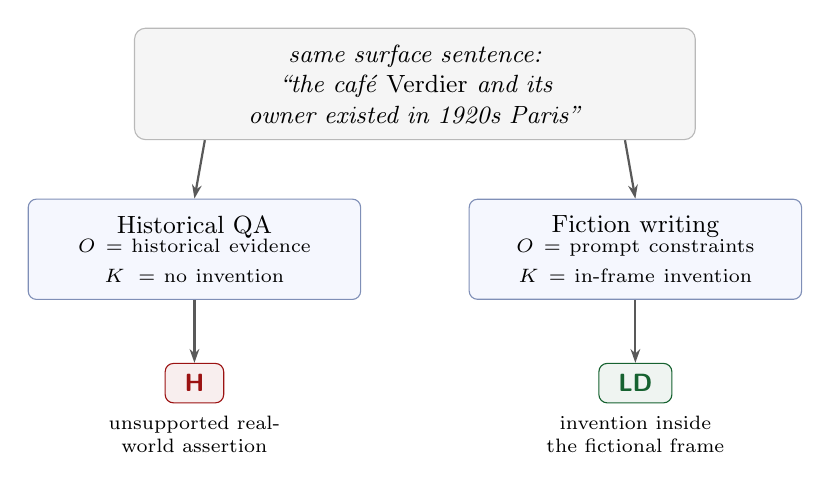
\begin{tikzpicture}[x=1cm,y=1cm]
  \node[input,text width=6.7cm] (s) at (0,0)
    {same surface sentence:\\``the caf\'e \emph{Verdier} and its owner existed in 1920s Paris''};
  \node[decision,text width=3.8cm] (qa) at (-2.8,-2.1)
    {Historical QA\\[-1pt]{\scriptsize $O=$ historical evidence\\$K=$ no invention}};
  \node[decision,text width=3.8cm] (fi) at (2.8,-2.1)
    {Fiction writing\\[-1pt]{\scriptsize $O=$ prompt constraints\\$K=$ in-frame invention}};
  \node[verdictH] (h) at (-2.8,-3.8) {\Hall};
  \node[verdictLD] (ld) at (2.8,-3.8) {\LD};
  \node[font=\scriptsize,align=center,text width=3.7cm] at (-2.8,-4.45)
    {unsupported real-world assertion};
  \node[font=\scriptsize,align=center,text width=3.7cm] at (2.8,-4.45)
    {invention inside the fictional frame};
  \draw[arrow] (s.south west) ++(0.9,0) -- (qa.north);
  \draw[arrow] (s.south east) ++(-0.9,0) -- (fi.north);
  \draw[arrow] (qa) -- (h);
  \draw[arrow] (fi) -- (ld);
\end{tikzpicture}}
\caption{\textbf{Contract-dependent evaluation of one surface sentence.}
Under historical QA, the invented caf\'e is an unsupported real-world assertion and receives \Hall.
Under fiction writing, the corresponding in-frame statement receives \LD.
The wording is fixed, but the discourse frame and truth contract differ.}
\label{fig:flip}
\end{figure}

\paragraph{Evidence and scope}
We support the position in two ways.
First, we map forty hallucination and creativity evaluation resources against the components of the proposed contract.
This mapping is purposive and single-coded; it identifies a pattern in the sample rather than estimating prevalence in the full literature.
Second, we apply the decision rule to four worked cases that isolate changes in evidence, permission, presentation, and scope.
These cases illustrate the intended behavior of the rule but do not establish annotation reliability or completeness.

\paragraph{Contributions}
This position paper makes three contributions.
First, it introduces a compact distinction between evidence status and task permission through $\TC(p)=(O_p,K_p)$, \Hall, and \LD.
Second, it maps a sample of factuality and creativity protocols to show where task permissions remain implicit.
Third, it proposes a research agenda for contract-aware benchmarks and mitigation methods that reduce \Hall\ without suppressing \LD.

\section{Truth Contracts and Claim-Level Verdicts}\label{sec:framework}

\subsection{Unit of analysis}

We use a claim-level unit because a single response may mix supported, unsupported, and non-propositional material \citep{min_factscore_2023,bayat_factbench_2024}.
Let $s$ denote a surface sentence and let $c(s,p)$ denote the proposition obtained by interpreting $s$ in the discourse established by prompt $p$.
This distinction matters for fiction, metaphor, and hypothetical language.
The same wording can yield different context-indexed propositions under different prompts.

Before assigning a factual verdict, an evaluator must decide whether an output span contributes a truth-conditional proposition.
Purely stylistic variation receives the label \SV.
This first step may require interpretation: metaphor and hyperbole cannot always be separated from propositional content by surface cues alone.

\subsection{The truth contract}

\textbf{Truth contract (\TC).}
For prompt $p$, the truth contract is
\[
  \TC(p)=(O_p,K_p), \qquad K_p=(m_p,\Gamma_p,\rho_p).
\]
The two components answer different questions.

\textbf{Reference evidence ($O_p$).}
$O_p$ is the evidence against which the claim is evaluated, such as a source document, retrieval set, database, gold labels, or a specified external reference.
The phrase ``world knowledge'' is only a shorthand; reproducible evaluation requires a concrete evidence source or an explicit adjudication procedure \citep{ji_survey_2023,bang_hallulens_2025}.

\textbf{Content-permission policy ($K_p$).}
$K_p$ specifies three properties:
\begin{itemize}
  \item $m_p$: the permission mode, such as grounded reporting, flagged speculation, or in-frame invention;
  \item $\Gamma_p$: the scope within which unsupported content is allowed;
  \item $\rho_p$: the required epistemic presentation, such as a hedge, an explicit hypothesis marker, or a declared fictional frame.
\end{itemize}
These modes are categorical rather than ordinal.
Flagged speculation is not simply a weaker version of fiction; it carries a different commitment and a different presentation requirement.

A strict grounded task has an empty permission scope for unsupported propositions.
A hypothesis-generation task may allow propositions within a stated topic if they are marked as provisional.
A fictional task may allow unhedged statements inside the declared fictional world while still prohibiting false claims about real people outside that frame \citep{searle_logical_1975}.

\subsection{Form condition}

We record a separate, three-level form condition $\sigma_p\in\{0,1,2\}$ that describes how much the requested wording may vary while preserving its propositions:
\begin{itemize}
  \item $\sigma_p=0$ (neutral/literal): minimal rhetorical transformation and no salient authorial voice;
  \item $\sigma_p=1$ (moderately marked): local metaphor, register shift, or a light stylistic voice while the intended propositions remain transparent;
  \item $\sigma_p=2$ (strongly marked): sustained figurative language, a salient voice, or substantial stylistic transformation.
\end{itemize}
The levels order degree of formal marking, not creativity or permission to invent.
Style is multi-dimensional, so this three-level scheme is a working discretization rather than a validated universal scale \citep{kang_style_2021,jin_deep_2022}.
The boundaries, especially between $\sigma_p=1$ and $\sigma_p=2$, require empirical validation.
The purpose of $\sigma_p$ is diagnostic: a factuality verifier may react differently to literal and figurative realizations of the same proposition.
Because $\sigma_p$ does not itself authorize a new proposition, it does not directly determine the \Hall/\LD\ verdict.
Failure to produce a requested style is an instruction-following error, not a truth-contract violation.

\subsection{Evidence state and verdict}

For every truth-conditional claim $c$, record the evidence relation
\[
E(c,O_p)\in\{\textsc{entailed},\textsc{contradicted},\textsc{unknown}\}.
\]
The last value means that the available evidence neither supports nor contradicts the claim.
Evidence state alone does not determine the contractual verdict.

Let $L(c,K_p)$ indicate whether mode $m_p$ licenses a non-entailed claim $c$ within scope $\Gamma_p$, and let $M(c,K_p)$ indicate whether its presentation satisfies $\rho_p$.
Then
\[
V(c\mid p)=
\begin{cases}
\SUP & \text{if }E(c,O_p)=\textsc{entailed},\\[1mm]
\LD & \text{if }E(c,O_p)\neq\textsc{entailed}\land L(c,K_p)=1\land M(c,K_p)=1,\\[1mm]
\Hall & \text{otherwise.}
\end{cases}
\]
Usefulness $U(c,p)$ is reported as a separate task-dependent score over \LD\ claims.
A low usefulness score does not change \LD\ into \Hall.

An explicit refusal or a statement such as ``the available evidence is insufficient'' is evaluated as a meta-claim about the evidence.
It is not automatically treated as asserting the embedded unsupported proposition.
This distinction prevents calibrated abstention from being mislabeled as hallucination.

Figure~\ref{fig:decision} summarizes the procedure.

\begin{figure*}[t]
\centering
\resizebox{0.93\linewidth}{!}{%
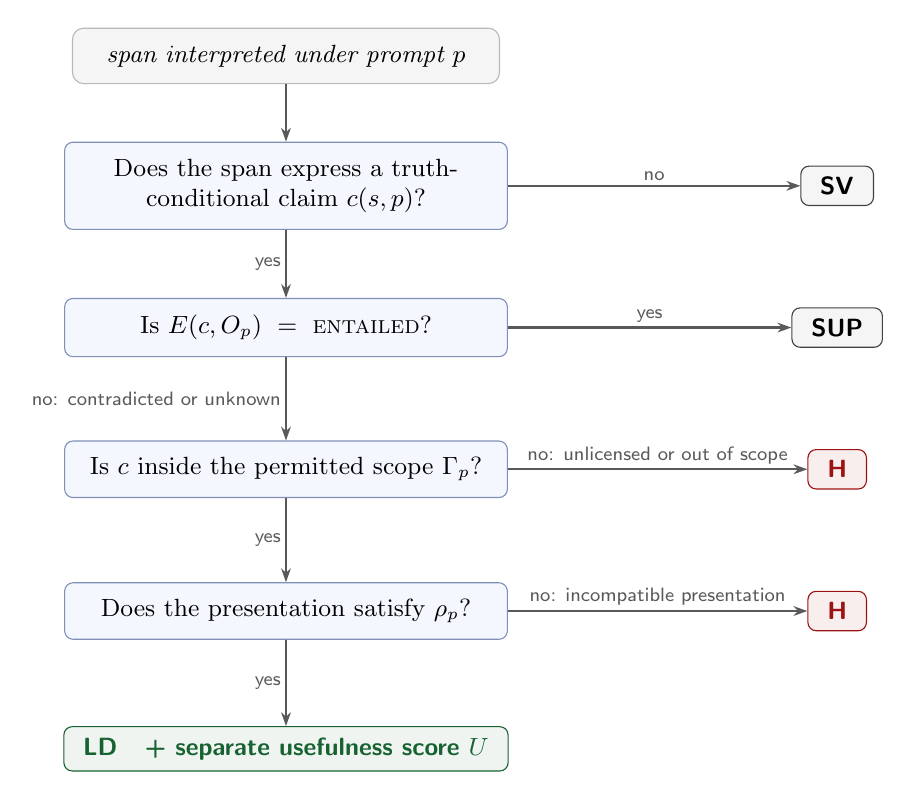
\begin{tikzpicture}[x=1cm,y=1cm]
  \node[input] (c) at (0,0) {span interpreted under prompt $p$};
  \node[decision] (q1) at (0,-1.65) {Does the span express a truth-conditional claim $c(s,p)$?};
  \node[decision] (q2) at (0,-3.45) {Is $E(c,O_p)=\textsc{entailed}$?};
  \node[decision] (q3) at (0,-5.25) {Is $c$ inside the permitted scope $\Gamma_p$?};
  \node[decision] (q4) at (0,-7.05) {Does the presentation satisfy $\rho_p$?};
  \node[verdict] (sv) at (7.0,-1.65) {\SV};
  \node[verdict] (sup) at (7.0,-3.45) {\SUP};
  \node[verdictH] (h1) at (7.0,-5.25) {\Hall};
  \node[verdictH] (h2) at (7.0,-7.05) {\Hall};
  \node[verdictLD] (ld) at (0,-8.8) {\LD\quad + separate usefulness score $U$};
  \draw[arrow] (c) -- (q1);
  \draw[arrow] (q1) -- node[edge,left]{yes} (q2);
  \draw[arrow] (q2) -- node[edge,left]{no: contradicted or unknown} (q3);
  \draw[arrow] (q3) -- node[edge,left]{yes} (q4);
  \draw[arrow] (q4) -- node[edge,left]{yes} (ld);
  \draw[arrow] (q1.east) -- node[edge,above]{no} (sv.west);
  \draw[arrow] (q2.east) -- node[edge,above]{yes} (sup.west);
  \draw[arrow] (q3.east) -- node[edge,above]{no: unlicensed or out of scope} (h1.west);
  \draw[arrow] (q4.east) -- node[edge,above]{no: incompatible presentation} (h2.west);
\end{tikzpicture}}
\caption{\textbf{Claim-level decision procedure.}
The evaluator first separates propositional content from stylistic variation and records the claim's relation to $O_p$.
A non-entailed claim receives \Hall\ if it falls outside the permitted scope or violates the required epistemic presentation; otherwise, it receives \LD.
Usefulness is attached to \LD\ as a separate score and is not a classification gate.}
\label{fig:decision}
\end{figure*}

\subsection{Representative contracts}

Table~\ref{tab:contracts} applies the rule to representative prompts.
Each row holds one contract fixed and evaluates one claim against it.

\begin{table*}[t]
\centering
\small
\setlength{\tabcolsep}{5pt}
\renewcommand{\arraystretch}{1.15}
\caption{\textbf{Representative truth contracts and claim-level verdicts.}
$O$ is the reference evidence; $K$ states the permission mode, scope, and required presentation.
Usefulness is reported separately for claims labeled \LD.}
\label{tab:contracts}
\begin{tabularx}{\linewidth}{@{}P{0.19\linewidth}P{0.19\linewidth}YP{0.06\linewidth}P{0.21\linewidth}@{}}
\toprule
\textbf{Prompt} & \textbf{Contract} & \textbf{Output claim} & \textbf{Label} & \textbf{Reason}\\
\midrule
Summarize this medical report & $O$: report; $K$: grounded only & The patient has diabetes (absent from the report) & \Hall & Unsupported and unlicensed\\
Explain photosynthesis like a poet, but keep the science accurate & $O$: scientific references; $K$: grounded only; $\sigma=2$ & Chlorophyll is a green workshop for sunlight & \SV & Figurative realization; no added scientific proposition\\
List possible causes and mark unestablished suggestions & $O$: available clinical evidence; $K$: flagged speculation in diagnostic scope & This could be early Lyme disease, but it requires testing & \LD & In scope and explicitly provisional\\
Write a story set in 1920s Paris & $O$: prompt constraints; $K$: in-frame invention & The fictional caf\'e Verdier opened at dawn & \LD & Invention inside the declared fictional world\\
Write a story set in 1920s Paris & $O$: prompt constraints plus historical references; $K$: in-frame invention & A real named person made a fabricated statement, presented as biography & \Hall & Real-world assertion outside the licensed frame\\
\bottomrule
\end{tabularx}
\end{table*}

\subsection{Relation to adjacent concepts}

Faithfulness asks whether a claim is supported by provided evidence, while factuality asks whether it is correct against an external reference \citep{maynez_faithfulness_2020,kryscinski_evaluating_2020}.
Both are evidence relations.
The content-permission policy asks a different question: what may the output do when the evidence does not entail a proposition?

Intent-aware evaluation is also related because it checks whether an output satisfies query constraints \citep{hao_faithqa_2025}.
However, general intent combines many requirements.
The truth contract isolates the subset that determines support, permission, scope, and epistemic presentation.

Recent work distinguishes potentially valuable or ``intelligent'' hallucinations from defective ones \citep{jiang_survey_2024,sui_confabulation_2024,yang_hicbench_2025}.
Our distinction is not based on output value alone.
Permission is evaluated before usefulness: an ingenious fabricated medical fact remains \Hall, while an unhelpful but in-frame fictional invention remains \LD\ with low usefulness.

\section{Evidence for a Diagnostic Gap}\label{sec:audit}

\subsection{Purposive mapping protocol}

We examined forty evaluation resources selected to span factual question answering, grounded generation, intent evaluation, creative writing, divergent thinking, and constrained problem solving.
The mapping is purposive rather than systematic.
It was designed to test whether prominent examples from both research traditions explicitly score the variables needed by the proposed contract.

For each resource, we recorded four questions:
\begin{enumerate}
  \item Does the protocol specify a reference evidence source?
  \item Does it vary or score the permission to introduce unsupported content?
  \item Does it represent the scope of that permission?
  \item Does it score the required epistemic presentation?
\end{enumerate}
We also recorded whether marked form is evaluated as a possible source of factuality-measurement error.

The current mapping was coded in one author pass.
The inferred task profiles are interpretive annotations, not measurements reported by the original resources.
Accordingly, our conclusion is limited to this sample and requires independent recoding before the mapping can be released as a validated resource.
Appendix~\ref{app:mapping} lists the resources and the inferred profiles.

\subsection{Observed pattern in the sample}

Table~\ref{tab:mapping-summary} summarizes the mapping at the level of resource groups.
The twenty-four strict factuality and faithfulness resources generally fix an evidence source and assume that unsupported propositions are errors.
The two closest intent or hallucination-taxonomy resources represent part of the problem but do not jointly score evidence, permission scope, and presentation.
The nine creative-generation resources generally assume permission to invent, while the five constrained creative-problem-solving resources add feasibility or correctness checks.
None of the forty resources in this purposive sample treats evidence, permission scope, and epistemic presentation as independent scored variables in one hallucination verdict.

\begin{table*}[t]
\centering
\small
\renewcommand{\arraystretch}{1.12}
\caption{\textbf{Summary of the purposive mapping of forty resources.}
The counts describe the author-coded sample, not the full literature.
``Implicit'' means that the task design appears to assume a value without scoring it as an independent variable.}
\label{tab:mapping-summary}
\begin{tabularx}{\linewidth}{@{}YP{0.06\linewidth}P{0.15\linewidth}P{0.16\linewidth}P{0.16\linewidth}P{0.16\linewidth}@{}}
\toprule
\textbf{Resource group} & \textbf{$n$} & \textbf{Reference $O$} & \textbf{Permission} & \textbf{Scope / presentation} & \textbf{Form control}\\
\midrule
Strict factuality / faithfulness & 24 & Usually fixed & Implicitly disallowed & Not varied & Not scored\\
Intent / hallucination taxonomy & 2 & Partial or task-dependent & Partly represented & Not jointly scored & Not scored\\
Creative generation / divergent thinking & 9 & Often absent or rubric-based & Implicitly allowed & Usually task-implied & Not used to condition factuality\\
Constrained creative problem solving & 5 & Feasibility, environment, tests, or soundness & Implicitly allowed & Partly constrained & Not used to condition factuality\\
\bottomrule
\end{tabularx}
\end{table*}

The sample also leaves an important off-diagonal setting underrepresented: strongly marked form under a strict factual contract.
Examples include ``explain this scientific result like a poet, but keep every claim accurate.''
Such tasks can reveal whether a factuality verifier mistakes figurative realization for unsupported propositional content.
This is a measurement hypothesis, not a result established by the present paper.

Figure~\ref{fig:profiles} organizes the target task profiles without treating permission modes as an ordinal scale.

\begin{figure*}[t]
\centering
\resizebox{0.96\linewidth}{!}{%
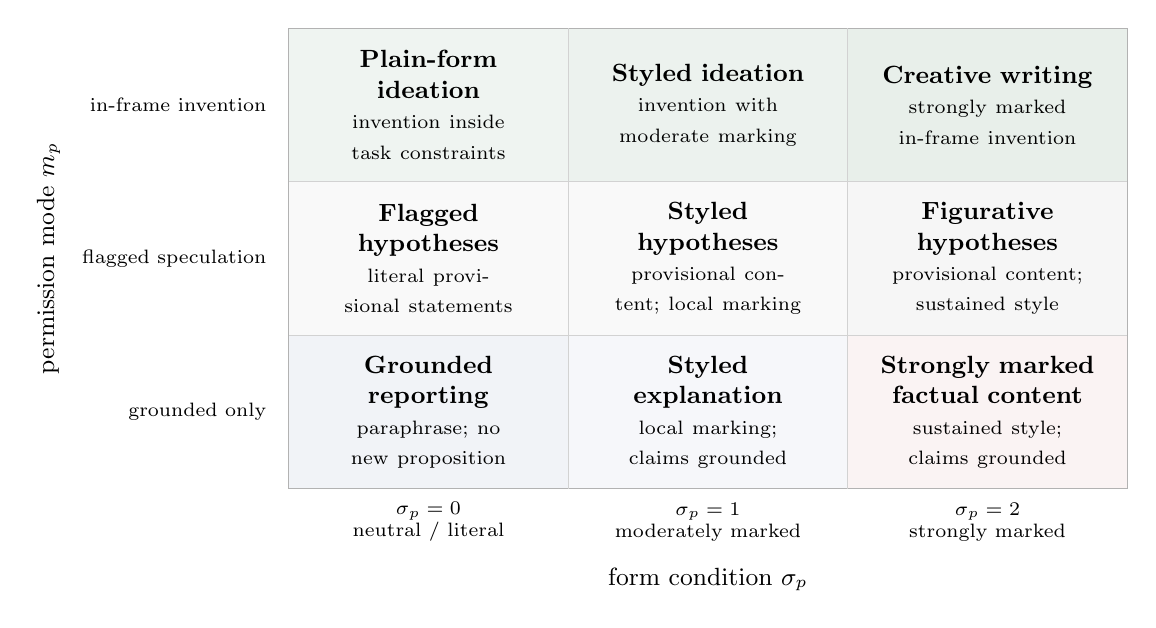
\begin{tikzpicture}[x=1cm,y=1cm,font=\small]
  \def\cw{3.55}
  \def\rh{1.95}
  \fill[clrB!6] (0,0) rectangle (\cw,\rh);
  \fill[clrB!4] (\cw,0) rectangle (2*\cw,\rh);
  \fill[clrH!5] (2*\cw,0) rectangle (3*\cw,\rh);
  \fill[gray!5] (0,\rh) rectangle (\cw,2*\rh);
  \fill[gray!5] (\cw,\rh) rectangle (2*\cw,2*\rh);
  \fill[gray!7] (2*\cw,\rh) rectangle (3*\cw,2*\rh);
  \fill[clrLD!7] (0,2*\rh) rectangle (\cw,3*\rh);
  \fill[clrLD!8] (\cw,2*\rh) rectangle (2*\cw,3*\rh);
  \fill[clrLD!10] (2*\cw,2*\rh) rectangle (3*\cw,3*\rh);
  \draw[gray!60] (0,0) rectangle (3*\cw,3*\rh);
  \draw[gray!35] (\cw,0)--(\cw,3*\rh);
  \draw[gray!35] (2*\cw,0)--(2*\cw,3*\rh);
  \draw[gray!35] (0,\rh)--(3*\cw,\rh);
  \draw[gray!35] (0,2*\rh)--(3*\cw,2*\rh);
  \node[align=center,text width=3.15cm] at (0.5*\cw,0.5*\rh)
    {\textbf{Grounded reporting}\\{\scriptsize paraphrase; no new proposition}};
  \node[align=center,text width=3.15cm] at (1.5*\cw,0.5*\rh)
    {\textbf{Styled\\explanation}\\{\scriptsize local marking; claims grounded}};
  \node[align=center,text width=3.15cm] at (2.5*\cw,0.5*\rh)
    {\textbf{Strongly marked\\factual content}\\{\scriptsize sustained style; claims grounded}};
  \node[align=center,text width=3.15cm] at (0.5*\cw,1.5*\rh)
    {\textbf{Flagged\\hypotheses}\\{\scriptsize literal provisional statements}};
  \node[align=center,text width=3.15cm] at (1.5*\cw,1.5*\rh)
    {\textbf{Styled\\hypotheses}\\{\scriptsize provisional content; local marking}};
  \node[align=center,text width=3.15cm] at (2.5*\cw,1.5*\rh)
    {\textbf{Figurative hypotheses}\\{\scriptsize provisional content; sustained style}};
  \node[align=center,text width=3.15cm] at (0.5*\cw,2.5*\rh)
    {\textbf{Plain-form ideation}\\{\scriptsize invention inside task constraints}};
  \node[align=center,text width=3.15cm] at (1.5*\cw,2.5*\rh)
    {\textbf{Styled ideation}\\{\scriptsize invention with moderate marking}};
  \node[align=center,text width=3.15cm] at (2.5*\cw,2.5*\rh)
    {\textbf{Creative writing}\\{\scriptsize strongly marked in-frame invention}};
  \node[font=\scriptsize,align=center] at (0.5*\cw,-0.42){$\sigma_p=0$\\neutral / literal};
  \node[font=\scriptsize,align=center] at (1.5*\cw,-0.42){$\sigma_p=1$\\moderately marked};
  \node[font=\scriptsize,align=center] at (2.5*\cw,-0.42){$\sigma_p=2$\\strongly marked};
  \node[font=\small] at (1.5*\cw,-1.15){form condition $\sigma_p$};
  \node[font=\scriptsize,anchor=east] at (-0.16,0.5*\rh){grounded only};
  \node[font=\scriptsize,anchor=east] at (-0.16,1.5*\rh){flagged speculation};
  \node[font=\scriptsize,anchor=east] at (-0.16,2.5*\rh){in-frame invention};
  \node[font=\small,rotate=90] at (-3.05,1.5*\rh){permission mode $m_p$};
\end{tikzpicture}}
\caption{\textbf{Task profiles across permission mode and form condition.}
Rows distinguish grounded reporting, flagged speculation, and in-frame invention; columns distinguish the three provisional form levels $\sigma_p\in\{0,1,2\}$.
The grid separates content permission from form and does not treat a higher $\sigma_p$ as permission to add unsupported propositions.}
\label{fig:profiles}
\end{figure*}

\subsection{Closest prior directions}

Intent hallucination evaluates whether a response omits or misinterprets query constraints \citep{hao_faithqa_2025}.
It therefore supports the broader claim that hallucination evaluation should consider the task rather than the output alone.
However, it does not provide the same separation between evidence relation and permission to depart from evidence.

HIC-Bench distinguishes intelligent and defective hallucinations using creativity and factual-deviation dimensions \citep{yang_hicbench_2025}.
This is close to the \LD/\Hall\ distinction, but its classification is driven by output scores.
Our proposed order is different: first determine whether the task licenses the departure, then evaluate the usefulness of licensed content.

The creativity-oriented hallucination literature argues that some unsupported generations can have creative value \citep{jiang_survey_2024,sun_hallucinating_2024,sui_confabulation_2024}.
The truth contract adds a normative boundary: potential value does not excuse a departure that the task did not permit.

\subsection{Why unsupported generation is not the target}

Formal work suggests that some errors remain possible for sufficiently general models operating with incomplete evidence \citep{kalai_calibrated_2024,xu_hallucination_2024,banerjee_llms_2024}.
This does not imply a constant error rate in deployment, and inevitability in the worst case can coexist with a very low practical probability \citep{suzuki_negligible_2025}.

More importantly for our position, reducing every departure from observed evidence would also restrict tasks that explicitly require hypotheses or invention.
The operational objective should therefore be to reduce unlicensed departures (\Hall) while preserving task-licensed departures (\LD).
Recent empirical work indicates that mitigation methods can affect divergent creativity differently, which motivates reporting both outcomes \citep{banerjee_does_2025,sun_hallucinating_2024}.

\section{Worked Contract Shifts}\label{sec:cases}

The following cases test one component at a time.
They are conceptual demonstrations rather than measurements.
Case A uses a documented summarization pattern; Cases B--D are constructed to isolate permission and scope.

\paragraph{Case A: changing the evidence reference}
In XSum, an extrinsic but factual summary statement may be absent from the source document while being correct against external evidence \citep{maynez_faithfulness_2020}.
With $O=$ source document and grounded-only $K$, the statement is unsupported and receives \Hall.
With $O=$ an external evidence set that entails the same proposition, it receives \SUP.
The surface text does not change; the evidence reference does.

\paragraph{Case B: changing the discourse frame}
The caf\'e sentence in Figure~\ref{fig:flip} is \Hall\ when interpreted as a real-world historical assertion under a grounded QA contract.
Under a declared fictional frame, the corresponding fictional-world proposition is in scope and receives \LD.
The example holds the wording fixed while changing its context-indexed interpretation and permission policy.

\paragraph{Case C: changing the required presentation}
Suppose the available evidence cannot determine whether a tool supports several input formats.
Under a grounded contract, presenting support as an established fact receives \Hall.
Under a hypothesis-generation contract, a qualified statement such as ``the tool may support several formats, but this requires version-specific verification'' can receive \LD.
The underlying possibility remains similar, but its licensed status and epistemic presentation differ.

\paragraph{Case D: testing a scope boundary}
A fictional frame does not license every false statement placed inside a story.
If a response attributes a fabricated biographical claim to a real named person and presents it as real history, the claim falls outside the fictional scope and remains \Hall.
Permission is limited by $\Gamma_p$.

\begin{table}[t]
\centering
\small
\setlength{\tabcolsep}{4pt}
\renewcommand{\arraystretch}{1.13}
\caption{\textbf{Worked cases illustrating contract-dependent verdicts.}
The table states which component changes and whether the result is \SUP, \LD, or \Hall.}
\label{tab:cases}
\begin{tabular}{@{}cP{0.26\columnwidth}P{0.29\columnwidth}P{0.29\columnwidth}@{}}
\toprule
\textbf{Case} & \textbf{Changed component} & \textbf{First condition} & \textbf{Second condition}\\
\midrule
A & Evidence $O$ & Source-only: \Hall & External evidence entails claim: \SUP\\
B & Frame and $K$ & Historical QA: \Hall & Fictional frame: \LD\\
C & Mode and presentation & Asserted as verified: \Hall & Licensed and flagged: \LD\\
D & Scope $\Gamma$ & In-frame invention: \LD & Real-world claim outside scope: \Hall\\
\bottomrule
\end{tabular}
\end{table}

\section{Research Agenda}\label{sec:agenda}

The framework identifies four empirical problems.

\textbf{1. Contract annotation and inference.}
Benchmarks should annotate the evidence reference, permission mode, permitted scope, and required epistemic presentation separately.
Because prompts can be ambiguous, benchmarks should preserve annotator disagreement rather than force one hidden default.
Future work must also model conflicts among user prompts, system instructions, domain rules, and safety policies.

\textbf{2. Reliable claim-level labeling.}
Evaluation requires a codebook for contextualized claim extraction, three-way evidence states, scope checks, and presentation checks.
Reliability should be reported for each layer because agreement on evidence does not imply agreement on permission boundaries.
Usefulness should remain a separate score with its own uncertainty \citep{acar_creativity_2019,marco_reader_2025}.

\textbf{3. Controlled benchmark design.}
A diagnostic benchmark should cross permission mode with the three form levels $\sigma_p\in\{0,1,2\}$ while holding propositional content as stable as possible.
This design would test whether contract annotation changes system rankings, whether verifier error varies monotonically with formal marking, and whether annotators can reliably distinguish the two boundaries.
The full mapping in Appendix~\ref{app:mapping} is a starting set of comparators, not a validated benchmark.

\textbf{4. Mitigation that preserves licensed divergence.}
Retrieval, verification, abstention, and constrained decoding should be evaluated on two outcomes: reduction of \Hall\ under grounded contracts and preservation of useful \LD\ under permissive contracts.
One aggregate hallucination rate cannot represent both objectives.

\section{Discussion}\label{sec:discussion}

\subsection{Evaluation implications}

Contract-aware evaluation separates claim-level verdicts from output-level objectives.
At claim level, a departure is supported, hallucinated, or licensed.
At output level, a response may still be too conservative for a creative task even when it contains no \Hall.
We call this an \emph{LD shortfall}: the response provides less licensed exploration than the task requires.
LD shortfall is not a fourth claim label because it concerns missing content rather than an observed claim.

The framework also separates verdict from severity.
A false drug dose and a wrong trivia date can both receive \Hall, but their costs differ.
Severity should weight the penalty after the contractual verdict rather than determine whether a violation occurred.

\subsection{Limitations}

The position has seven main limitations.
First, contract specification is partly normative: reasonable evaluators may disagree about the correct evidence source and permission boundary.
Second, the framework is prompt-centered, although real systems also follow system instructions, policies, and multi-turn context.
Third, claim extraction under metaphor, irony, hypothesis, and fiction remains difficult.
Fourth, the three-level $\sigma_p$ scheme is a provisional discretization whose thresholds and annotation reliability have not been validated.
Fifth, the \LD\ rule and usefulness score have not been validated with human annotation.
Sixth, the mapping is purposive and single-coded, so it cannot support prevalence claims about the full literature.
Seventh, a user's permission does not override safety, legal, or domain constraints; contract inference must therefore identify which instruction source has authority.

These limitations define empirical work rather than invalidate the distinction.
Making disagreement and authority explicit is preferable to hiding them inside a default factuality protocol.

\section{Conclusion}\label{sec:conclusion}

Hallucination is not a context-free property of a sentence.
It is a claim-level verdict relative to the evidence and permissions of a task.
The proposed truth contract, $\TC(p)=(O_p,K_p)$, separates the reference evidence from the content-permission policy.
An unsupported claim is \Hall\ when it violates that policy and \LD\ when it falls within the permitted scope and uses the required epistemic presentation.
Usefulness and severity are evaluated separately.
The three-level form condition $\sigma_p$ remains a diagnostic variable for testing verifier robustness and does not itself license new content.

The purposive mapping shows that none of the forty resources in our sample jointly scores evidence, permission scope, and epistemic presentation as independent components of one hallucination verdict.
The worked cases illustrate why those components can change the appropriate label.
The next step is empirical: validate contract annotation, measure whether it changes evaluation outcomes, and test mitigation methods on both \Hall\ reduction and \LD\ preservation.

\appendix

\appendixsection{Formal Decision Rule}\label{app:formal}

For a surface span $s$ produced under prompt $p$, let $c(s,p)$ be its context-indexed proposition when one exists, and let $\sigma_p\in\{0,1,2\}$ record neutral/literal, moderately marked, or strongly marked form.
Non-propositional material receives \SV\ and exits the factual decision rule.
For a propositional claim, define
\[
E(c,O_p)\in\{\textsc{entailed},\textsc{contradicted},\textsc{unknown}\},
\]
let $r(c)$ denote the claim's surface realization, and let
\begin{align*}
L(c,K_p)&=\mathbb{1}[m_p\text{ licenses }c\text{ within }\Gamma_p],\\
M(c,K_p)&=\mathbb{1}[r(c)\text{ satisfies }\rho_p].
\end{align*}
The verdict is
\[
V(c\mid p)=
\begin{cases}
\SUP & E(c,O_p)=\textsc{entailed},\\
\LD & E(c,O_p)\neq\textsc{entailed}\land L(c,K_p)=1\land M(c,K_p)=1,\\
\Hall & E(c,O_p)\neq\textsc{entailed}\land\bigl(L(c,K_p)=0\lor M(c,K_p)=0\bigr).
\end{cases}
\]
Usefulness is a separate, task-dependent score $U(c,p)$ defined by the evaluation protocol.

The central claim concerns a fixed surface sentence interpreted under two contracts:
\[
\exists s,p_1,p_2:\quad
V(c(s,p_1)\mid p_1)=\Hall
\quad\land\quad
V(c(s,p_2)\mid p_2)=\LD.
\]
This statement concerns contract-dependent verdicts, not relative truth.

\appendixsection{Resource Mapping}\label{app:mapping}

Tables~\ref{tab:full-mapping-factual} and~\ref{tab:full-mapping-creative} list the forty resources used in the purposive mapping.
The task profiles are author annotations inferred from the original protocols.
They should be independently recoded before release as a validated dataset.

\begin{table*}[t]
\centering
\scriptsize
\setlength{\tabcolsep}{4pt}
\renewcommand{\arraystretch}{0.98}
\caption{\textbf{Factuality, faithfulness, and adjacent resources in the purposive mapping.}
``Grounded'' means that unsupported claims are implicitly disallowed; ``in-frame'' means that invention is task-implied; ``partial'' marks resources that represent only part of the proposed contract.
These are author-coded profiles, not labels reported by the original resources.}
\label{tab:full-mapping-factual}
\begin{tabular}{@{}P{0.31\textwidth}P{0.18\textwidth}P{0.19\textwidth}P{0.23\textwidth}@{}}
\toprule
\textbf{Resource} & \textbf{Task} & \textbf{Reference evidence} & \textbf{Author-coded profile}\\
\midrule
\multicolumn{4}{l}{\textbf{Strict factuality and faithfulness}}\\
FEVER \citep{thorne_fever_2018} & Fact checking & Wikipedia evidence & Grounded\\
TruthfulQA \citep{lin_truthfulqa_2022} & Factual QA & External factual reference & Grounded\\
PopQA \citep{mallen_when_2023} & Long-tail QA & Wikidata & Grounded\\
SimpleQA \citep{wei_measuring_2024} & Factual QA & External factual reference & Grounded\\
TriviaQA \citep{joshi_triviaqa_2017} & Reading QA & Evidence documents & Grounded\\
DefAn \citep{rahman_defan_2024} & Factual QA & External factual reference & Grounded\\
HaluEval \citep{li_halueval_2023} & QA and summarization & World/reference context & Grounded\\
FactBench \citep{bayat_factbench_2024} & Factual QA & Retrieved evidence & Grounded; includes undecidable\\
HalluLens \citep{bang_hallulens_2025} & Factual QA & Task-specific evidence & Grounded\\
FRANK \citep{pagnoni_understanding_2021} & Summarization & Source documents & Grounded\\
QAGS \citep{wang_asking_2020} & Summarization & Source documents & Grounded\\
SummEval \citep{fabbri_summeval_2021} & Summarization & Source documents & Grounded\\
XSum \citep{narayan_xsum_2018} & Summarization & BBC source & Grounded\\
CNN/DailyMail \citep{hermann_teaching_2015} & Summarization & News source & Grounded\\
DelusionQA \citep{sadat_delucionqa_2023} & Domain QA & Manuals & Grounded\\
HaluQA \citep{cheng_evaluating_2023} & Long-form QA & External factual reference & Grounded\\
BIG-Bench \citep{srivastava_beyond_2023} & Multi-task reasoning & Task gold & Grounded\\
BIG-Bench Hard \citep{suzgun_challenging_2023} & Reasoning & Task gold & Grounded\\
CR-LLM \citep{li_cr-llm_2024} & Concept reasoning & Gold concepts/context & Grounded\\
HotpotQA \citep{yang_hotpotqa_2018} & Multi-hop QA & Wikipedia & Grounded\\
HypoTermQA \citep{uluoglakci_hypotermqa_2024} & Hypothetical QA & Task/world reference & Grounded\\
HalluRAG \citep{ridder_hallurag_2025} & RAG QA & Retrieved Wikipedia & Grounded\\
ToolQA \citep{zhuang_toolqa_2023} & Tool-use QA & Tools and APIs & Grounded\\
RealTimeQA \citep{kasai_realtime_2024} & Real-time QA & Current evidence & Grounded\\
\midrule
\multicolumn{4}{l}{\textbf{Closest intent and hallucination taxonomies}}\\
FaithQA \citep{hao_faithqa_2025} & Intent verification & Query constraints & Partial: intent constraints\\
HIC-Bench \citep{yang_hicbench_2025} & Hallucination typing & Task-dependent & Partial: intelligent/defective\\
\bottomrule
\end{tabular}
\end{table*}

\begin{table*}[t]
\centering
\scriptsize
\setlength{\tabcolsep}{4pt}
\renewcommand{\arraystretch}{0.98}
\caption{\textbf{Creativity and constrained problem-solving resources in the purposive mapping.}
The profiles are author annotations inferred from task design, not variables reported by the original resources.}
\label{tab:full-mapping-creative}
\begin{tabular}{@{}P{0.31\textwidth}P{0.18\textwidth}P{0.19\textwidth}P{0.23\textwidth}@{}}
\toprule
\textbf{Resource} & \textbf{Task} & \textbf{Reference evidence} & \textbf{Author-coded profile}\\
\midrule
\multicolumn{4}{l}{\textbf{Creative generation and divergent thinking}}\\
CreativityPrism \citep{hou_creativityprism_2025} & Multi-task creativity & Rubrics & In-frame invention\\
LitBench \citep{fein_litbench_2025} & Story evaluation & Human preferences & In-frame invention\\
Short Story \citep{ismayilzada_evaluating_2025} & Story generation & Semantic/human criteria & In-frame invention\\
WritingBench \citep{wu_writingbench_2025} & Creative writing & Rubric/human criteria & In-frame invention; style scored\\
Art-or-Artifice / TTCW \citep{chakrabarty_art_2024} & Creative writing & Expert rubric & In-frame invention\\
Automated DT scoring \citep{organisciak_beyond_2023} & Divergent thinking & Automated rubric & In-frame invention\\
Verbal Creativity \citep{dinu_testing_2025} & Divergent thinking & TTCT & In-frame invention\\
Automated Creativity \citep{li_automated_2025} & Creative writing & Reference texts & In-frame invention\\
Hallucinating Narratives \citep{sun_hallucinating_2024} & Controlled story/reasoning & Mixed & In-frame invention; mixed support\\
\midrule
\multicolumn{4}{l}{\textbf{Constrained creative problem solving}}\\
MacGyver \citep{tian_macgyver_2025} & Problem solving & Human feasibility & Invention plus feasibility\\
EscapeBench \citep{qian_escapebench_2025} & Agent puzzles & Environment state & Invention plus correctness\\
CreativEval \citep{delorenzo_creativeval_2024} & Code generation & Specification/tests & Invention plus correctness\\
NeoCoder \citep{lu_benchmarking_2025} & Code generation & Unit tests & Invention plus correctness\\
Math Creativity \citep{ye_assessing_2024} & Math problem solving & Human soundness & Invention plus soundness\\
\bottomrule
\end{tabular}
\end{table*}

\bibliography{references}

\end{document}
